\section{Appendix A: Speed of Sound}

Sound wave is a pressure disturbance that moves with at a speed $a$

\begin{figure}[h!]
	\centering
	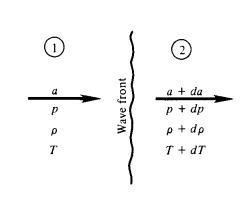
\includegraphics[width=0.3\linewidth]{screenshot001.png}
	\caption{}
	\label{fig:screenshot001}
\end{figure}

By applying a rectangular control volume around this pressure wave, we can apply our conservation equations. We are assuming that these properities are increasing by a small increment. This is why each variable is added by a infinitesimally small term.

Recalling the conservation of mass (continuity equation), $\dot{m} = constant$

\[\dot{m}_{left} = \dot{m}_{right}\]

Recalling he definition of density, $\rho = m/\bar{V}$ and rewriting $\bar{V} = uA$ (check the units)
\[\rho a \cancel{A}  = (\rho + d\rho)(a + da) \cancel{A}\]
Futher expanding gives,
\[\rho a   = (\rho a+ \rho da + a d\rho + da d\rho)\]

We say that $da d\rho$ is so small, we can assume it is zero. This is often referred to as "neglecting higher order terms (H.O.T)". The expression then becomes

\[\frac{da}{a} = -\frac{d \rho}{\rho}\]

For the momentum equation $P + \rho u^2 = constant$
\[P + \rho a^2  = P + dP +  (\rho + d\rho)(a + da)(a + da) \]

But we just said that $\rho a = (\rho + d\rho)(a + da)$


\[P + \rho a^2  = P + dP +  \rho a(a + da) \]
\[dP + \rho ada = a\]

Multiplying the second term by a and divide by a, this is essentially multiplying the second term by one.

\[dP + \rho a^2\frac{da}{a} = a\]

recalling the relation $\frac{da}{a} = -\frac{d \rho}{\rho}$

\[dp - a^2 d \rho = 0\]

                       \[a^2 = \frac{dp}{d\rho}\]

Since a sound wave is a very weak wave, when it travels through a medium, it only increases the pressure and density, etc. slightly. The effect of this is that friction  and heat transfer can be neglected. Since friction cannot be undone, we call this an irreversible process. Whenever there is no transfer of heat, it is called this adiabatic. Thus, the propagation of sound is an adiabatic, reversible process, otherwise called isentropic. Isentropic implies no increase in entropy, which is \textit{not} true in the presence of shock waves.

In the case of a thermally perfect gas, we can say $P = \rho R T$

For a callorically perfect gas we can say $pv^{\gamma} = constant$, where $v$ is volume per unit mass, or specific volume

Differentiating and recalling that $v = 1/\rho$

\[a = \sqrt{\frac{\gamma P}{\rho}} = \sqrt{\gamma R T}\]


\[dm = \left( \rho u\right)_2 - \left(\rho u\right)_1\]
\[D(mV) = \left(\rho u^2 + P \right)_2\]

For Steady flow,

\[\cancel{dm} = \left( \rho u\right)_2 - \left(\rho u\right)_1\]

\[ \left( \rho u\right)_1 = \left(\rho u\right)_2\]

Similarly, for the Momentum equation,

\[\left(\rho u^2 + P\right)_1 = \left(\rho u^2 + P\right)_2\]

Let us change the coordinate system motion for the traveling wave be independent of time, and thus corresponds to \textit{steady state} wave propagation. 
\[ u_1 = \bar{u} + a - \frac{1}{2} \partial u \]
\[ u_2 = \bar{u} + a + \frac{1}{2} \partial u \]


where, $\bar{u}$ is the average flow velocity and $a$ is the wave speed.


Substituting this back into the conservation of mass

\[\left(\rho u\right)_1 = \left(\rho u\right)_2 \]

\[ 
\left( \rho    - \frac{1}{2}\partial \rho \right) 
\left( \bar{u} - a - \frac{1}{2}\partial u\right) = 
\left( \rho    + \frac{1}{2}\partial \rho \right) 
\left( \bar{u} - a + \frac{1}{2}\partial u\right) 
\]

Further expanding

\[
\cancel{
	\rho \bar{u} - \rho a
} + 
\frac{1}{2} 
\left(
-\rho \partial u - \bar{u} - \bar{u} \partial \rho + a \partial \rho 
\right) +
\cancel{
	\frac{1}{4}\partial \rho \partial u 
}
= 
\cancel{
	\rho \bar{u} - \rho a
} + 
\frac{1}{2} 
\left(
\rho \partial u + \bar{u} - \bar{u} \partial \rho - a \partial \rho 
\right) +
\cancel{
	\frac{1}{4}\partial \rho \partial u 
}
\]
 
\[
  \frac{1}{2}\left( - \rho \partial u - \bar{u} \partial \rho + a \partial \rho\right) = 
  \frac{1}{2}\left(   \rho \partial u + \bar{u} \partial \rho - a \partial \rho\right)
\]

\[
\rho \partial u + u \partial \rho - a \partial \rho = 0 
\]

\[
\rho \partial u + \left( u - a\right)\partial \rho = 0
\]

Momentum Equation

\[
\left(\rho u^2 + P\right)_1 = 
\left(\rho u^2 + P\right)_2\]



